\documentclass{standalone}
\usepackage{tikz}
\usetikzlibrary{calc, patterns}

\usepackage{amssymb, amsmath}
\usepackage[]{ifthen}

\def\ex{.5}
\def\ey{8/3}

\def\xlo{-3}
\def\xhi{5}
\def\ylo{-2}
\def\yhi{5}
\begin{document}
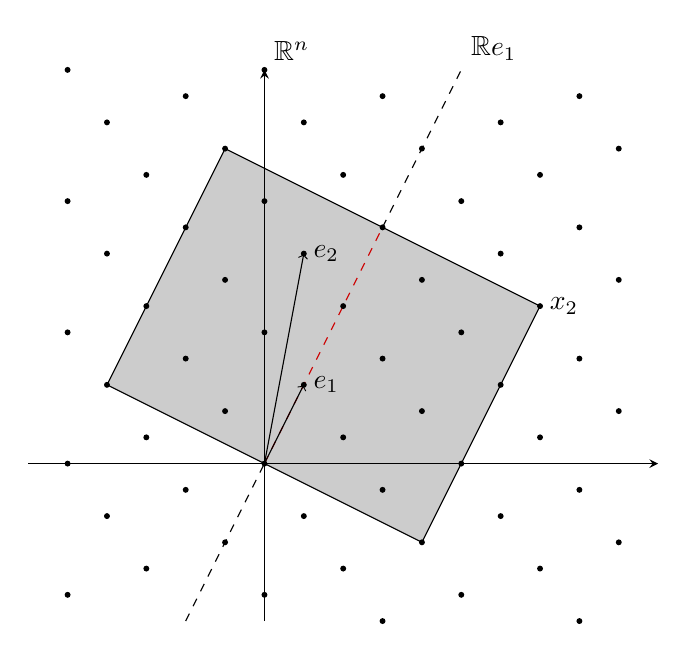
\begin{tikzpicture}
	\draw[fill = gray!40!white] (3.5,2) -- (-.5,4) -- (-2,1) -- (2,-1) -- cycle;
	\draw[-stealth] (\xlo,0) -- (\xhi,0);
	\draw[-stealth] (0,\ylo) -- (0,\yhi) node[anchor = south west] {\(\mathbb{R}^n\)};
	\draw[dashed] (-1,-2) -- (0,0);
	\draw[dashed, red!80!black] (0,0) -- (1.5,3);
	\draw[dashed](1.5,3) -- (2.5,5) node[anchor = south west] {\(\mathbb{R} e_1\)};
%	\draw[dashed,,postaction={-, draw=green,dash pattern=on 0pt off 2.24cm on 3.35cm off 7.83cm}] (0,0) -- (1.5,3) node[anchor = south west] {\(\mathbb{R} e_1\)};
	\draw[-to] (0,0) -- (.5,1) node[anchor = west] {\(e_1\)};
	\node[anchor = west] at (3.5,2) {\(x_2\)};
	\foreach \i in {-20,...,20}{
		\foreach \j in {-20,...,20}{
			\pgfmathparse{.5*\i + \ex*\j < \xhi ? 1:0}
			\ifthenelse{\pgfmathresult > 0}{
				\pgfmathparse{abs(\ey*\j + \i) < \yhi ? 1:0}
				\ifthenelse{\pgfmathresult > 0}{
					\pgfmathparse{.5*\i + \ex*\j > \xlo ? 1:0}
					\ifthenelse{\pgfmathresult > 0}{
						\pgfmathparse{\ey*\j + \i > \ylo ? 1:0}
						\ifthenelse{\pgfmathresult > 0}{
							\draw[fill] (.5*\i + \ex*\j,\ey*\j + \i) circle (.03);
						}{}
					}{}
				}{}
			}{}
		}
 	}
	\draw[-to] (0,0) -- (\ex,\ey) node[anchor = west] {\(e_2\)};
\end{tikzpicture}
\end{document}